\section{Summative analysis}\label{sec:summative}

As was discussed in Section~\ref{subsec:structure}, the vast majority of our
attributes will not be considered at this stage of our analysis so we can focus
on how the cost of care is distributed and seen in the data. The exclusion of
these attributes does not, however, imply that they are not of interest. 

\subsection{Distributions and summative
statistics}\label{subsec:distributions_statistics}
\graphicspath{{./img/general/}}

When we look at the distributions of our subset of attributes on the whole
dataset we see that the data is skewed towards low-cost, short-stay, and
otherwise low-impact patients with long, heavy tails, as seen in
Figures~\ref{fig:netcost_kde}~\--~\ref{fig:no_spells_hist}. We can then take
advantage of the other attributes to identify slices of the dataset which are of
interest by literature review, clustering, or otherwise.

\begin{figure}[h!]
    \centering
    \begin{minipage}{.495\textwidth}
        \includegraphics[width=\linewidth]{netcost_kde/main.pdf}
        \captionof{figure}{Estimated probability density for the net cost of a
        spell, clipped at \pounds12,500.}\label{fig:netcost_kde}
    \end{minipage}\hfill%
    \begin{minipage}{.495\textwidth}
        \includegraphics[width=\linewidth]{los_hist/main.pdf}
        \captionof{figure}{Histogram for the total length of a spell, clipped at
        21 days.}\label{fig:los_hist}
    \end{minipage}
\end{figure}

In this section, and subsequently, when we refer to `spell-level' quantities, we
mean that each of our cost components and the number of procedures are summed
over all episodes in any given spell, the number of diagnoses at the spell level
is considered as the maximal number of diagnoses in a spell, and the length of
stay is unique to the spell not the episode. The decision to take the maximal
number of diagnoses as opposed to the total number of diagnoses is justified
since, (a.) we want to minimise the effect of counting the same diagnosis more
than once at the spell level, and (b.) the severity of a patient's condition is
often compared against their Charlson~comorbidity~index~(CCI), which a weighted
summation of their individual severities~\cite{Thygesen2011}. As such, by taking
the maximum number of diagnoses we hope to capture the most severe a patient's
condition becomes during a spell as this is often indicative of how aggressive
the patient's treatments are, and thus likely more expensive due to additional
drug or ward costs, for instance.

\begin{figure}[h!]
    \centering
    \begin{minipage}{.495\textwidth}
        \includegraphics[width=\linewidth]{no_diag_hist/main.pdf}
        \captionof{figure}{Histogram for the number of diagnoses in an
        episode.}\label{fig:no_diag_hist}
    \end{minipage}\hfill%
    \begin{minipage}{.495\textwidth}
        \includegraphics[width=\linewidth]{no_proc_hist/main.pdf}
        \captionof{figure}{Histogram for the number of procedures in an
        episode.}\label{fig:no_proc_hist}
    \end{minipage}
\end{figure}

As can clearly be seen, the dataset has some significant skew. In particular,
the average lengths and total number of stays for patients are low
(Figures~\ref{fig:los_hist}~\&~\ref{fig:no_spells_hist} respectively). A
corollary to be drawn from these plots is that it seems that of all the spells
in hospital provided under the health board, the majority of them are daycases
and one-off treatments.

\begin{figure}[h!]
    \centering
    \begin{minipage}{.495\textwidth}
        \includegraphics[width=\linewidth]{no_spells_hist/main.pdf}
        \captionof{figure}{Histogram for the number of spells associated with a
        patient.}\label{fig:no_spells_hist}
    \end{minipage}\hfill%
    \begin{minipage}{.495\textwidth}
        \includegraphics[width=\linewidth]{age_hist/main.pdf}
        \captionof{figure}{Histogram for the age of patients with two-year
        bins.}\label{fig:age_hist}
    \end{minipage}
\end{figure}

However, this does not imply that these spells all come cheap. When we look at
the distribution of the net cost of a spell (Figure~\ref{fig:netcost_kde}) we
see that although there is a distinct peak around a relatively low net cost,
this value has probability \(7.5\times10^{-4}\ (2 sf.)\). That is, the most
likely net cost of treating a patient in this dataset occurs less than one tenth
of a percent of the time, and the overwhelming majority of recorded net costs
are spread over a massive range. While tests do exist for verifying if our
empirical data is truly heavy-tailed~\cite{Bryson1974}, it is clear our net
costs (at least) are distributed in such a way. Further results on the
distributions of our net and component costs can be seen in
Table~\ref{tab:summative}.

\begin{table}[h!]
    \resizebox{\textwidth}{!}{%
        \begin{tabular}{lrrrrrrrrrr}
\toprule
{} &       COST &       CRIT &      DRUG &      EMER &      ENDO &       HCD &       IMG &   IMG\_OTH &        MED &       NCI \\
\midrule
mean &    1834.93 &     -92.08 &     75.40 &      1.24 &     21.19 &     20.91 &     32.70 &     20.57 &     347.12 &    -30.92 \\
std  &    3771.16 &    1332.61 &    315.17 &     29.13 &     92.76 &    210.98 &    143.67 &    118.26 &     739.73 &     85.80 \\
min  &       4.50 & -250000.61 &     -0.57 &      0.00 &      0.00 &      0.00 &      0.00 &      0.00 &       0.00 & -12960.21 \\
25\%  &     347.67 &       0.00 &      7.18 &      0.00 &      0.00 &      0.00 &      0.00 &      0.00 &      44.45 &    -29.75 \\
50\%  &     749.49 &       0.00 &     20.00 &      0.00 &      0.00 &      0.23 &      0.08 &      0.00 &     130.67 &    -11.64 \\
75\%  &    1886.38 &       0.00 &     59.88 &      0.00 &      0.00 &      4.83 &     10.93 &      0.31 &     375.32 &     -3.02 \\
max  &  369168.93 &       0.00 &  63430.52 &  33347.89 &  11855.95 &  94411.85 &  46708.66 &  46708.66 &  116449.90 &      0.00 \\
\bottomrule
\end{tabular}

    }
    \resizebox{\textwidth}{!}{%
        \begin{tabular}{lrrrrrrrrrr}
\toprule
{} &       NID &    NetCost &     OCLST &       OPTH &      OTH &  OTH\_OTH &      OUTP &        OVH &      PATH &  PATH\_OTH \\
\midrule
mean &     94.83 &    1742.85 &     13.30 &     160.11 &     1.37 &     0.97 &      0.57 &     354.82 &     36.20 &     23.29 \\
std  &    248.16 &    3185.31 &     58.74 &     486.24 &    11.67 &    10.15 &     26.79 &     734.05 &    135.47 &    122.71 \\
min  &      0.00 &       4.50 &      0.00 &       0.00 &     0.00 &     0.00 &      0.00 &       0.00 &      0.00 &      0.00 \\
25\%  &     14.99 &     347.32 &      0.00 &       0.00 &     0.00 &     0.00 &      0.00 &      84.86 &      0.00 &      0.00 \\
50\%  &     32.25 &     747.13 &      0.77 &       0.00 &     0.00 &     0.00 &      0.00 &     139.47 &      4.63 &      0.00 \\
75\%  &     83.36 &    1862.51 &      5.43 &       0.04 &     0.00 &     0.00 &      0.00 &     320.93 &     31.89 &     13.76 \\
max  &  84374.21 &  369168.93 &  12358.37 &  111396.20 &  1248.83 &  1248.83 &  10632.15 &  106428.61 &  70008.12 &  70008.12 \\
\bottomrule
\end{tabular}

    }
    \resizebox{\textwidth}{!}{%
        \begin{tabular}{lrrrrrrrrrr}
\toprule
{} &  PATH\_OTH &      PHAR &  PROC\_NO &      PROS &   RADTH &     SECC &       SPS &       THER &  TRUE\_LOS &       WARD \\
\midrule
mean &     23.29 &     30.47 &     1.90 &     40.71 &    0.65 &     0.87 &     11.81 &      28.62 &      2.90 &     497.07 \\
std  &    122.71 &     86.70 &     2.21 &    343.57 &    8.01 &    27.43 &    149.46 &     181.58 &      9.21 &    1236.63 \\
min  &      0.00 &      0.00 &     0.00 &      0.00 &    0.00 &     0.00 &      0.00 &       0.00 &      0.00 &       0.00 \\
25\%  &      0.00 &      2.26 &     0.00 &      0.00 &    0.00 &     0.00 &      0.00 &       0.09 &      0.00 &      10.33 \\
50\%  &      0.00 &      7.24 &     1.00 &      0.00 &    0.00 &     0.00 &      0.00 &       0.63 &      0.00 &     142.01 \\
75\%  &     13.76 &     26.21 &     3.00 &      0.00 &    0.00 &     0.00 &      0.00 &      10.49 &      2.00 &     463.04 \\
max  &  70008.12 &  25087.73 &    70.00 &  33930.70 &  227.64 &  2177.74 &  68029.58 &  125249.49 &   3659.00 &  203854.11 \\
\bottomrule
\end{tabular}

    }
    \caption{Summative spell-level statistics for each of our non-trivial cost
    components and our selected clinical variables.}\label{tab:summative}
\end{table}

There are methods available to attempt to overcome this skewedness, including
the scaling and transformation of our numerical attributes, but they are not
necessary for the purposes of a summative analysis, though this process could
improve the performance of several algorithms on the dataset since it is of
mixed type. Moreover, the presence of this skewedness in some attributes is not
to say that all the attributes are so harshly skewed; for instance,
Figure~\ref{fig:age_hist} shows the clear peaks and troughs in the distribution
of the ages of our patients. It is clear that the distribution of ages does not
have a bell-shaped curve and should likely not be modelled as normally
distributed \-- or otherwise `bell-shaped', for that matter.

\subsection{Pairwise correlation}\label{subsec:corr}

Figure~\ref{fig:corr_heatmap} shows the Pearson correlation coefficient of all
pairs in our subset of selected attributes (not including age or number of
spells) in the form of a heatmap with a colour bar is located to the right of
it. Using a visual aid such as this makes gaining insight from our array of
numbers, and thus the relationships between our variables, much easier than
studying a table or matrix directly. It should also be noted that these
attributes are considered at the spell level again.

\begin{figure}[h!]
    \vspace{-50pt}%
    \includegraphics[width=1.2\textwidth]{corr_heatmap/main.pdf}
    \caption{A heatmap of the pairwise correlation coefficients for our cost
    components, and our other clinical attributes.}\label{fig:corr_heatmap}
\end{figure}

Upon inspection of Figure~\ref{fig:corr_heatmap}, we see that there are several
cost components, such as secondary commisioning costs (SECC) and emergency care
(EMER), that have no significant linear correlation with any of the other
attributes. While there seems to be an abundance of non-correlation across the
heatmap, there are clear correlations between many of our attributes; some of
these are easier to realise than others. For instance, ignoring the main
diagonal, the largest value is that between total costs (COST) and net costs at
\(0.94\). This indicates almost total positive linear correlation between these
two variables, and that makes sense given that our net cost is just the total
cost corrected for a number of reimbursable costs like critical care (CRIT)
and non-contracted income (NCI) which are entered as negative values in the
dataset \-- hence the distinctly negative correlation coefficients they have
with the other variables. Typically, these costs are small (see
Table~\ref{tab:summative}) so we would expect a strong correlation between costs
and net costs.

Another example is the strong correlation amongst the length of stay
(TRUE\_LOS), and ward and overhead costs (WARD and OVH respectively). We can
justify these anecdotally: the longer a patient spends in hospital, the more
time they are likely to spend on a ward and incurring associated overheads like
administration work and cleaning costs. It should also be clear that these
attributes all share a strong linear correlation with the net cost of a spell.
This implies that these costs and the length of stay are good indicators of the
net cost of treating someone, and may suggest that the cost components make up a
substantial and relatively consistent part of the net cost.

\subsection{Measuring variation and importance in our cost components}

The purpose of this entire work is to understand the factors leading to
variations in the cost of treating someone in hospital so it is fitting to look
at the constituent parts of our net cost: the cost components. In this section
we will make use of a dimensionless measure of variation for, and the mean
contribution to the net cost of, each cost component during a spell. Using these
pairs of quantities, we can compare the components against one another in an
rudimentary way.

During a preliminary analysis of our cost components, it was found that our
conclusions on the variations in each component were misled owing to the fact we
were measuring variation using the unbiased sample variance. While this quantity
is a perfectly valid unbiased estimator for the population variance, it is
entirely dependent on the scale of the attribute being considered. This
dependency is evident in Table~\ref{tab:summative}. In place of this measure we
use the coefficient of variation which is the ratio between the standard
deviation and mean, and so is scale invariant.

\begin{definition}
    Consider a population with mean \(\mu\) and standard deviation \(\sigma\).
    Then the \emph{coefficient of variation} is defined to be:

    \[
        C_{v} := \frac{\sigma}{\mu}
    \]

    If only a sample of the data from a population is available then the
    coefficient of variation can be estimated using the sample standard
    deviation and the sample mean analogously.
\end{definition}

In Figure~\ref{fig:cost_variation}, the coefficient of variation for each of our
cost components is shown as a bar in a bar chart. The components have been
ranked in descending order of their variations and it clear that there are a
number of strongly variant attributes. Taking secondary commisioning costs
(SECC) again, we see that its standard deviation is over thirty times the size
of its mean. This alone could explain why there seemed to be no linear
correlation with the other variables in Figure~\ref{fig:corr_heatmap} since the
values for these costs are so wildly varied. At the other end of the scale we
see that our ward and overhead costs are amongst the attributes with the
smallest variation, implying that they are consistent as was supposed in
Section~\ref{subsec:corr}. Despite this, we can conclude that these attributes
are quite highly varied when considering the entire dataset since the majority
of coefficients of variation found have size far greater than one.

\begin{figure}[h]
    \centering
    \includegraphics[width=\textwidth]{cost_variation/main.pdf}
    \caption{Bar chart showing the coefficient of variation \(C_{v}\) of each
    cost component, and the net and total costs, in descending
    order.}\label{fig:cost_variation}
\end{figure}

At this point, knowing which of the cost components are the most highly varied
is not enough. To determine the relative importance of these findings, the
contribution of each cost component to the net cost of a spell must be
considered. After all, we only care for the components that make a significant
impact. We calculate these quantities by taking each cost component in turn,
dividing it by its corresponding net cost and taking the mean over all of these
values. We refer to this mean as the average contribution (or proportion) to the
net cost, although it is more accurately an average of the ratios between each
component and the net cost.

\begin{figure}[h]
    \centering
    \includegraphics[width=\textwidth]{cost_contribution/main.pdf}
    \caption{Bar chart showing the average contribution of each cost component
    to the net cost of a spell, in descending
    order.}\label{fig:cost_contribution}
\end{figure}

By inspecting Figure~\ref{fig:cost_contribution}, it is seen that, on average,
ward and overhead costs are the two largest contributors to the net cost of a
spell. This is then followed by medical costs (MED) before the average
contribution drops down to roughly \(5\%\) and below for the various
department-specific cost components. Then for our most varied components in
Figure~\ref{fig:cost_variation}, we see their average contribution to net cost
is effectively negligible in comparison to the majority of our other components.

\begin{figure}[h]
    \centering
    \includegraphics[width=\textwidth]{cost_bubble_plot/main.pdf}
    \caption{A bubble plot showing the average contribution to the net cost of a
    spell along the vertical, and the coefficient of variation for that
    component as the size of its marker.}\label{fig:cost_bubble_plot}
\end{figure}

So, we can conclude that these components are not especially important. But what
about the others? The midriff of each of these plots contain many of the same
components. In order to aid understanding and interpretability of how these two
quantities relate to one another we make use of a bubble plot. Since each of the
plots are two-dimensional and can share the same horizontal axis, both of the
values can be visualised together by using the vertical axis and size as two
separate dimensions, as illustrated in Figure~\ref{fig:cost_bubble_plot}.

Figure~\ref{fig:cost_bubble_plot} can be interpreted either by first reading
along the vertical axis to find the components that make the most considerable
contribution to treating a patient and then investigating the relative variation
that component holds intrinsically in the dataset by looking at the size of its
outer marker. The reverse of this process is also perfectly logical since the
objective is to determine where the variation exists, and then how much of an
impact that has on the net cost. The latter is how
Figures~\ref{fig:cost_variation}~\&~\ref{fig:cost_contribution} we interpreted
above. The crux of interpreting this plot is that the further away a large
marker is from the zero line, the more important that component is considered.
However, small markers are also of interest since these components indicate that
the level of variation is relatively low \-- the reasons as to why unknown.

It is easily seen from this figure that our previous conclusions can still be
interpreted; that is, our largest contributors have some of the smallest
measures of variation while the smallest average contributors are more strongly
varied. What is of interest is the jump between these groups of cost components.
There does not seem to be any particular component in the midriff of
contributors that has huge, or indeed small, variation. As a result of this,
perhaps more investigation is needed into individual components and their
relationships with specific types of patient.

Also, the skewedness of our data could be having an adverse effect on the
representation of the last three plots, particularly those considering the
contribution to net cost. As was discussed earlier, this measure is not strictly
the contribution a component makes to the net cost since in some cases certain
components sum up to several multiples of the total net cost of the spell. This
is true in cases where critical care costs are taken as huge deductions from the
total cost of most the other components.

\subsection{Conclusions}

\textcolor{red}{%
    Overall conclusions and lead into the next chapter on diabetic patient
}
